\chapter{Introduction}\label{c1}
The protagonist in this thesis, deoxyribonucleic acid (\textbf{DNA}) was first isolated~\cite{nuclein} in 1869 by F. Miescher, and following several indispensable breakthroughs, its double-stranded helical structure was finally deciphered by J. Watson and F. Crick in 1953~\cite{dnastruc}.
The Watson-Crick model describes dsDNA as a helical structure with a sugar-phosphate bi-chain, also known as Crick and Watson strands, on the outside, held together by hydrogen-bonding between nitrogenous base-pairs inside.
This base-pairing is highly specific (Adenine[A]:Thymine[T], Guanine[G]:Cytosine[C]), so that either strand has the necessary information to replicate itself and is thus capable of transferring information from one generation to the next.
Nevertheless, the story did not end there.
Contemporary to the discovery of DNA structure, Conrad H. Waddington found that environmental factors also influence phenotypic features in fruit flies~\cite{epigenotype} and termed it \say{\textbf{epigenetics}} which means \say{in addition to genetics}.
It is formally defined as \say{An epigenetic trait is a stably heritable phenotype resulting from changes in a chromosome without alterations in the DNA sequence}~\cite{berger2009operational}.
The most common epigenetic modifications include base modifications, non-coding RNAs, and histone modifications.  
For instance, around 70-80\% of \cpg steps in mammalian cells~\cite{jabbari2004cytosine} are methylated and in promoter regions, it is anti-correlated with gene expression~\cite{cedar2009linking,pennings2005dna}.
Epigenetics has implications in gene silencing~\cite{kass1997does,cedar2009linking,pennings2005dna}, X-chromosome inactivation~\cite{goto1998regulation}, and in humans, epigenetic aberrations are associated with diseases such as cancer, autoimmune disease, and neurodevelopmental disorders~\cite{portela2010epigenetic,kulis2010dna} and, therefore, is of great interest for research.
Moreover, some epigenetic aberrations are reversible and, thus, targeted in therapeutic approaches~\cite{kelly2010epigenetic}.

With DNA as the protagonist, ribonucleic acid (\textbf{RNA}) is the deuteragonist.
It acts as a genetic carrier in viruses and has other diverse roles in biology such as reaction catalysis, genetic information processing, and gene regulation~\cite{mandal2004gene,fire1998potent,vsponer2006computational}.
Chemically, RNA only differs from DNA in deoxyribose sugar and Thymine, instead has ribose sugar and Uracil (U) base. 
In biology, RNA is often present in a single-stranded form; however, double-stranded RNA is also vital in gene regulation via RNA interference (sequence-specific gene suppression)~\cite{fire1998potent}, components of several tertiary structures such as riboswitches~\cite{mandal2004gene}, hairpins, and transfer RNA and as the genome of some viruses.
Moreover, in many biological processes~\cite{adams2012biochemistry,vella1994molecular,rich1960hybrid,brambati2020dark,meselson1958replication,shaw2008recognition}, unique heterogeneous nucleic acids (NAs) are formed with one DNA strand and one RNA strand known as DNA:RNA hybrid (\textbf{DRH}).
For example, during reverse transcription, RNA viruses create transient DRH whose stability is consequential in their replication cycle~\cite{vella1994molecular,brambati2020dark,marin2019sequence}.
Furthermore, DRHs are considered as potential medicinal agents for HIV or other retroviruses diseases~\cite{tisdale1991mutations,shaw2008recognition} and are crucial in the CRISPR-Cas9 technology~\cite{sternberg2015conformational}, genome stability, and DNA repair~\cite{ohle2016transient}.

In parallel, it became evident that not only the chemistry but also the mechanics of double-stranded nucleic acids, specifically their shape and flexibility, plays a crucial role in their function.
For example, DNA mechanics is pivotal in nucleosome positioning~\cite{segal2006genomic,segal2009controls}, indirect readout~\cite{chen2001indirect,napoli2006indirect}, DNA looping~\cite{schleif1992dna,adhya1989multipartite,basu2021measuring} and protein-DNA interactions~\cite{chen2001indirect,napoli2006indirect,rohs2009role,paillard2004analyzing,juo1996proteins}.
In particular, owing to its quintessential role in DNA readout, sequence-dependent mechanics of DNA is often regarded as a \say{secondary genetic code}.
Moreover, epigenetic modifications in DNA further regulate gene expression, supposedly by changing the mechanics of DNA.
For instance, methylation of \cpg steps in promoter regions leads to gene silencing~\cite{cedar2009linking,pennings2005dna} by reducing flexibility and, thus, reducing the ability of DNA to interact with transcription factors, modulating DNA accessibility and making them less prone to wrap around nucleosomes~\cite{cortini2016physics,perez2012impact,portella2013understanding,hognon2019cooperative,rohs2010origins}.
Sequence-dependent mechanics is also determining in the functioning of RNA and DRH as well~\cite{shaw2008recognition,stein1969enzyme,yesselman2019sequence,noy2005structure,suresh2014dna,noy2008theoretical}.
Such direct evidence piqued significant interest in understanding the sequence-dependent mechanics of nucleic acids.

The primary experimental tools for studying the mechanics of dsNAs are cyclization experiments~\cite{cycle1}, optical tweezers~\cite{optical1}, small-angle X-ray scattering~\cite{pollack2}, and cryogenic electron microscopy~\cite{cryoem,demurtas2009bending}.
More details on various techniques for \textit{in vivo} and \textit{in vitro} characterization of dsNAs mechanics can be found in ref.~\cite{peters2010dna}.
Even though experiment is an excellent approach to explore the role of mechanical properties of dsNAs in their functioning, designing and performing experiments is highly time-consuming and, thus, can only be performed for a few sequences.
Recently, Basu et al.~\cite{basu2021measuring} developed high-throughput methods to measure the tendency for DNA looping and computed intrinsic cyclizabilities of roughly 300,000 50 base-pairs (bps) DNA fragments (flanked both sides by 25 bps fixed duplex and single-stranded complementary overhangs) and found an intricate role of sequence in the overall mechanics of DNA that can not be sufficiently described by basic sequence descriptors such as GC content, A-tracts, and dimer steps.
Such experimental methods can provide an overall picture, but lack a finer description.

A promising alternative is provided by computational modeling and simulation.
In particular, atomistic molecular dynamics (MD) simulations have been widely used to study various structural, mechanical, and functional aspects of nucleic acids~\cite{marin2019sequence,hospital2015molecular,noy2005structure,suresh2014dna,noy2008theoretical,pasi2014muabc,dixit2005molecular,lankavs2003dna,battistini2021impact,carvalho2014understanding,perez2004relative,fujii2007sequence,perez2012impact,perez2008towards,perez2007dynamics,balaceanu2019modulation,orozco2003theoretical} and have become an indispensable tool in general for studying bio-molecules~\cite{hospital2015molecular}.
However, due to the immense sequence space of DNA, it is not feasible to investigate all sequences (even for DNA dodecamers); for instance, the most extensive analysis using atomistic MD simulations published so far is only for the 136 independent tetramers~\cite{pasi2014muabc,dixit2005molecular} by the ABC consortium.
Also, MD simulations are extremely slow for simulating longer dsNA fragments as most of the simulation time are consumed to model relatively uninteresting water molecules.
Therefore, a systematic investigation requires computationally efficient alternatives.

There have been several attempts to model DNA, starting with worm-like chain models~\cite{kratky1949,shimada1980statistical}. 
One of the first and widely applied models for the coarse-grained sequence-dependent DNA model was a rigid base-pair model~\cite{xraydata} with dimer-dependent parameters obtained from X-ray crystal data from protein-DNA complexes (which have been a great source of information to study the structure and flexibility of DNA~\cite{neidle2021beyond}).
Similar rigid base-pair models were also trained on atomistic MD simulations~\cite{lankavs2003dna,gonzalez2001extracting}.
One major drawback of rigid base-pair models is that the non-local sequence dependence in the model requires non-local sequence-dependent parameters, which are almost impractical to obtain, particularly for a model trained on experimental data.
Therefore, most rigid base-pair models only have local dimer sequence dependence.
However, it has been observed multiple times that sequence dependence limited to the local dimer step is not always sufficient to explain all properties of specific DNA sequences, and non-local sequence dependence (i.e., depend on flanking sequence) plays a pivotal role in DNA mechanics~\cite{fujii2007sequence,perez2008towards,balaceanu2019modulation,lavery2010systematic,yanagi1991analysis,packer2000sequence,arauzo2005sequence}.
In particular, Balaceanu et al.~\cite{balaceanu2019modulation} using MD simulations demonstrated that the structure and flexibility of the central TA step are significantly modulated by hexamer or even beyond flanking context.

More recently, a few other models have been proposed to study sequence-dependence properties in DNA~\cite{ouldridge2011structural, chakraborty2018sequence,3spn,dnamartini}; however, the parameters in these models have often been fit analytically to experimental data and have limited and local sequence-dependence.
The first and only model, to our knowledge, that predicts non-local sequence dependence in the shape of DNA is cgDNA~\cite{petkevivciute2014cgdna,cgDNA1}. cgDNA is a coarse-grained model of B-DNA which predicts the probability distribution function of an arbitrary DNA sequence (in standard A, T, C, G alphabets) under pre-specified physical solvent conditions. 
Originally, in this model, DNA was coarse-grained as a bi-chain of explicit bases, which is now extended to \say{cgDNA$+$}~\cite{patelithesis} with explicit representation of phosphates in addition to the bases.
The non-local sequence-dependence in the cgDNA($+$) model using dimer-dependent parameters originates from the fact that individual base-pair steps cannot achieve their local minima simultaneously, and frustration of energy surfaces arises in the nearest neighbors; thus, the cgDNA($+$) model naturally captures the non-local sequence-dependence in the DNA mechanics, but only using dimer dependent parameters.
Both models are trained on molecular dynamics time-series of a comprehensive set of DNA sequences, and the model predictions are shown to be almost indistinguishable from the corresponding MD statistics of first and second moments.


The cgDNA($+$) model has been successfully implemented to explore sequence-dependent persistence lengths~\cite{cgdnamc} of DNA, sequence-dependent unwrapping pathways of DNA from the nucleosome core particle~\cite{pollack-cgDNA}, crystal structure packing forces~\cite{patelithesis}, and the role of histone tails in nucleosome stability~\cite{bendandi2020role}.
Moreover, the cgDNA$+$ model has been used to scan entire genomes searching mechanically exceptional sequences~\cite{zwahlenthesis} and obtain sequence-dependent shapes of DNA minicircles~\cite{glowackithesis,beaud2021using}. 
Other exciting applications of the cgDNA$+$ model actively pursued (in LCVMM and with collaborators) include the response of DNA to external loading and twisting, the calculation of the nucleosome wrapping energy for DNA, and the prediction of protein-DNA binding affinity.
Moreover, this model can potentially contribute to fine-tuning rapidly evolving DNA applications, for example, DNA nanotechnology.
Thus, the model has shown great potential for diverse applications involving DNA mechanics with the overarching goal of deciphering how DNA mechanics facilitate its functioning in biology.

One particular limitation is that the current model only allows standard DNA bases.
However, in biology, bases in the DNA sequences are often modified, particularly, Cytosine (C), which is either methylated or hydroxymethylated at the $5$-position of Cytosine in \cpg steps.
Furthermore, RNA and DRH are also ubiquitous in biology and essential for several other applications.
Therefore, in this thesis, we have extended the cgDNA$+$ model by estimating parameter sets for RNA, DRH, and DNA with base modifications and called it the cgNA$+$ model.
Moreover, we have compared cgNA$+$ model predictions with experimental findings, particularly with the existing protein-DNA X-ray structure database for dimers in all tetramer flanking contexts, and further emphasized the model's potential to help understand the functioning of DNA in biology.
Another limitation is that the cgNA$+$ model treats sugar rings implicitly and does not provide any information on sugar pucker modes and backbone conformations. 
Notably, unlike phosphate and base groups, the sugar groups can not be treated as rigid bodies due to their high intrinsic flexibility.
Therefore, we have introduced a machine learning approach that predicts the position of all sugar atoms from the knowledge of position of neighboring phosphate and base atoms which can be obtained from the cgNA$+$ model.

This thesis has been divided into eight chapters. 
The first two chapters are dedicated to background material with basic details of nucleic acids in \cref{c1} and the description of the prior cgDNA$+$ model in \cref{c2} including the discussion of model training, various methods to assess the model, and the Monte Carlo code to sample from the predicted Gaussian pdf. 
In \cref{c3}, we have reported the MD simulation protocol and the training library used to parameterize the model. 
Furthermore, we have analyzed the various aspects of MD simulations performed for various nucleic acids.
In particular, we have examined the convergence of MD simulations and the distributions of cgNA$+$ internal coordinates for various nucleic acids. 
In \cref{c4}, we have introduced the cgNA$+$ model with a systematic assessment of the model's predictive capabilities.
Furthermore, we have applied the cgNA$+$ model to explore various applications of the cgNA$+$ model, such as computing persistence length and groove widths, and comparing the statistics for DNA, RNA, and DRH.
Moreover, we have also compared cgNA$+$ predictions with the available protein-DNA X-ray structure database in \cref{c5}.
In \cref{c6}, we have discussed the extension of the cgNA$+$ model for epigenetically modified bases, along with the illustration of various applications.
In \cref{c7}, we have introduced a neural network module to predict the location of sugar atoms in any cgNA$+$ coarse-grained configuration from the knowledge of neighboring base and phosphate atomic positions.
It allows computing sequence-dependent backbone conformations and sugar pucker modes for an arbitrary DNA sequence where the positions of base and phosphate atoms can be accurately obtained from the cgNA$+$ model.
Finally, \cref{c8} discusses the conclusions of this thesis, outlines limitations, and proposes directions for future work. 

\section{Nucleic acids}\label{c1:s2}
%https://casegroup.rutgers.edu/lnotes/dnab.pdf
% https://pubchem.ncbi.nlm.nih.gov//edit3/index.html
\begin{figure}[htb]
	\begin{center}
	\centering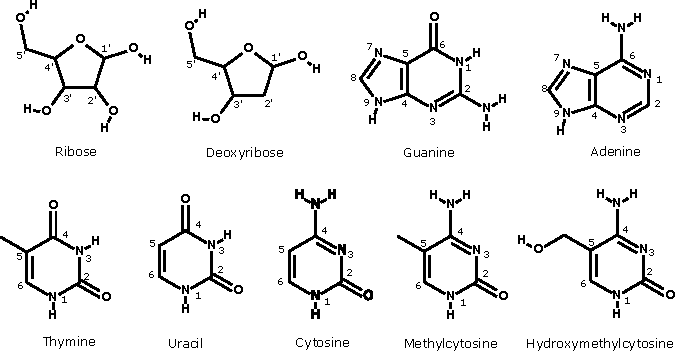
\includegraphics[scale=1.1]{images/combine_bases_final.pdf}
	\centering\caption{Chemical structure and labeling of various sugar and bases in nucleic acids.}
\label{c1:fig1}
\end{center}
\end{figure}

In this section, we describe the basic structural and chemical aspects of various NAs modeled in this thesis. 
A NA is a polymer of repeating nucleotides composed of three basic units: phosphate, sugar, and bases.
The sugar in NA is 5-carbon sugar (pentose) which is ribose and deoxyribose (as shown in \cref{c1:fig1}) in the case of RNA and DNA, respectively.
The sugar and phosphate are alternately connected through a phosphodiester bond and make the NA backbone (see \cref{c1:fig3}).
The phosphate group is attached to the $5^\prime-$ and $3^\prime-$ carbon of the pentose sugar that provides directionality to the NA, and the corresponding ends of the NA are called $5^\prime-$ and $3^\prime-$ ends.
Bases, the third component of NAs, are nitrogenous base compounds that act as elemental units of the genetic code. 
There are primarily two nucleobases categories: purine (R) and pyrimidine (Y) bases.
Purine bases are larger with two fused ring structures, while pyrimidine has a single ring.
The canonical purine bases are Adenine (A) and Guanine (G), while canonical pyrimidine bases are Thymine (T),  Cytosine (C), and Uracil (U) (as shown in \cref{c1:fig1}).
The base is connected to the sugar, forming an N-glycosidic bond between base-nitrogen (N1 for Y and N9 for R) and $1^\prime-$ carbon of the sugar ring.

\begin{figure}[htb]
	\begin{center}
	\centering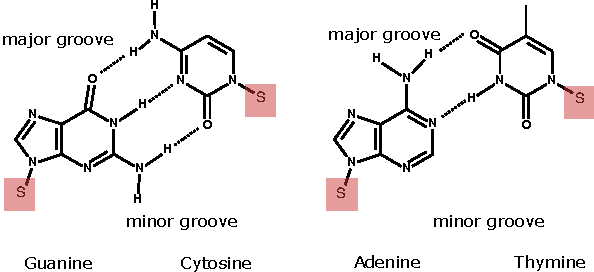
\includegraphics[scale=0.85]{images/base-pair.pdf}
	\centering\caption{Base-pairing and grooves in DNA
	}
\label{c1:fig2}
\end{center}
\end{figure}

Double-stranded NA (dsNA), which is the primary focus of this thesis, is composed of two such anti-parallel chains which
interact through the bases in which purine bases in one chain form hydrogen bonds with pyrimidine bases in other or vice-versa as shown in \cref{c1:fig2}. 
The direction of one chain is $5^\prime-$ to $3^\prime-$ end while $3^\prime-$ to $5^\prime-$ end for the other.
These interacting bases (through H-bonds) in the anti-parallel strands are complementary.
The following discussion is relevant to dsNA.

Now, the structure of dsNA is defined at four levels, namely, primary, secondary, tertiary, and quaternary.
The primary structure of a dsNA is defined as the list of nucleotides (denoted using the base name) read in the $5^\prime-$ to $3^\prime-$ end direction.
To write down this sequence of nucleotides ($\sq$), one of the strands is selected as the reading (or Watson) strand, while the other strand is called the complementary (or Crick) strand.
A dsNA oligomer comprising  of $N$ base-pairs as $\sq = X_1X_2X_3...X_{N-1}X_N$ where $X_i$ are in the alphabets representing bases and the sequence is written in the $5'$ to $3'$ direction.
The complementary base of $X_i$ on the Crick strand is $\bar{X}_{i}$.
Following the notation, $\bar{\sq}$, is written as $\bar{X}_N\bar{X}_{N-1}\bar{X}_{N-2}...\bar{X}_2\bar{X}_1$ in the $5'$ to $3'$ direction on the Crick strand. 
The secondary structure defines the interactions between the bases and, thus, defines the basic shape of dsNA. 
For example, in canonical dsNA, the complementary base-pairing and wrapping of the two strands lead to a double-helical structure.
There may be other types of secondary structures, such as bulges and loops but they are outside the scope of this thesis. 

The main interest in this work is the tertiary structure of dsNA which refers to its intrinsic shape and flexibility.
The tertiary structure includes key structural features, including handedness of the helix (left or right), length of helix per turn, the number of base-pairs per turn, and size of major and minor grooves.
These features depend mainly on the physical conditions and the type and sequence of dsNA. 
Finally, the quaternary structure of dsNAs describes their interactions with other molecules, e.g., protein-DNA complexes or interactions of different RNAs in the ribosome.
The following subsections provide basic information on the various dsNAs studied in this work.

\begin{figure}[htb]
	\begin{center}
	\centering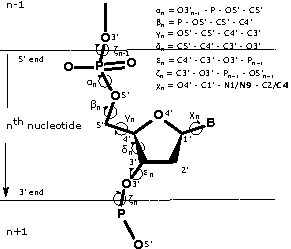
\includegraphics[scale=1.7]{images/backbone.pdf}
	\centering\caption{DNA backbone and the torsional angles as defined in ref.~\cite{schneider1997conformations}. 
	For $\chi_n$, the third and fourth atoms of the torsional angle depend on the kind of base. For pyrimidine bases, the atoms are N1 and C2, while for purine bases, the atoms are N9 and C4 as shown in bold.
	In the figure, the base is denoted as B.
	}
\label{c1:fig3}
\end{center}
\end{figure}
\subsection{Deoxyribonucleic Acid}\label{c1:s2:sb1}



The three components of a DNA nucleotide are deoxyribose sugar, phosphate, and bases (A, T, C, and G), as shown in \cref{c1:fig1}.
In the case of double-stranded DNA (dsDNA), complementary bases on opposite strands form H bonds, as shown in \cref{c1:fig2}.
In this base-pairing, C forms three H-bonds with G while A forms two H-bonds with T.
Furthermore, the distance between the backbones of two strands is not symmetrical and forms two grooves of different sizes called major and minor grooves, as shown in \cref{c1:fig2}.
The major and minor grooves arise because the glycosidic bonds (base-sugar bonds) in the base-pair are not diametrically opposite. 
Notably, for a given base-pair, the minor groove contains O2 of Y and N3 of R, and the major groove is on the opposite side.
Moreover, the methyl group of Thymine also lies in the major groove.
Each groove consists of potential H-bond donor and acceptor atoms that enable specific interactions with proteins, and the sequence modulates their precise chemistry. 
Thus, the sequence-dependent groove widths play a crucial role in the protein-DNA interaction~\cite{rohs2010origins,rohs2009role,oguey2010understanding,stofer1994measuring}. 

The sugar-phosphate backbone is, in general, quite flexible and therefore requires more parameters to characterize its conformations.
In \cref{c1:fig3}, we have shown a typical DNA backbone and standard torsional angles used to characterize its conformation.
It requires six torsional (or dihedral) angles (defined as the angle between planes passing through two sets of three atoms that have two atoms in common) to describe the backbone of DNA. 
In this case, the two sets of three atoms are consecutive first three and last three of the four covalently bonded atoms as described in \cref{c1:fig3}. 
Furthermore, there is an additional torsional angle involving base and sugar atoms called $\chi$. 
The involved base atoms depend on the type of base (R or Y) and are indicated in \cref{c1:fig3}.
$\chi$ torsional angle determines the nucleoside conformation, namely anti and syn. 
For anti conformation, $\chi \in [+90^\circ \cdots +270^\circ]$ while for the rest of the $\chi$ values, nucleoside is in the syn conformation. 
Primarily, nucleoside stays in anti-conformation but sometimes base flips from anti-to-syn conformation, known as base-flipping.
We would like to emphasize that the six torsional parameters in the DNA backbone are not entirely free to rotate and are quite restricted by steric constraints.
In particular, there exist two common backbone conformations B\rom{1} and B\rom{2}, which are inter-convertible. 
These B\rom{1}-B\rom{2} conformations are found to play an important role in protein-DNA recognition~\cite{gorenstein1994conformation}.
B\rom{1} or B\rom{2} conformation is identified by using the difference between the torsional angle $\epsilon-\zeta$ which is negative for the B\rom{1} conformation and positive for the B\rom{2} conformation.

\begin{figure}[H]
	\begin{center}
	\centering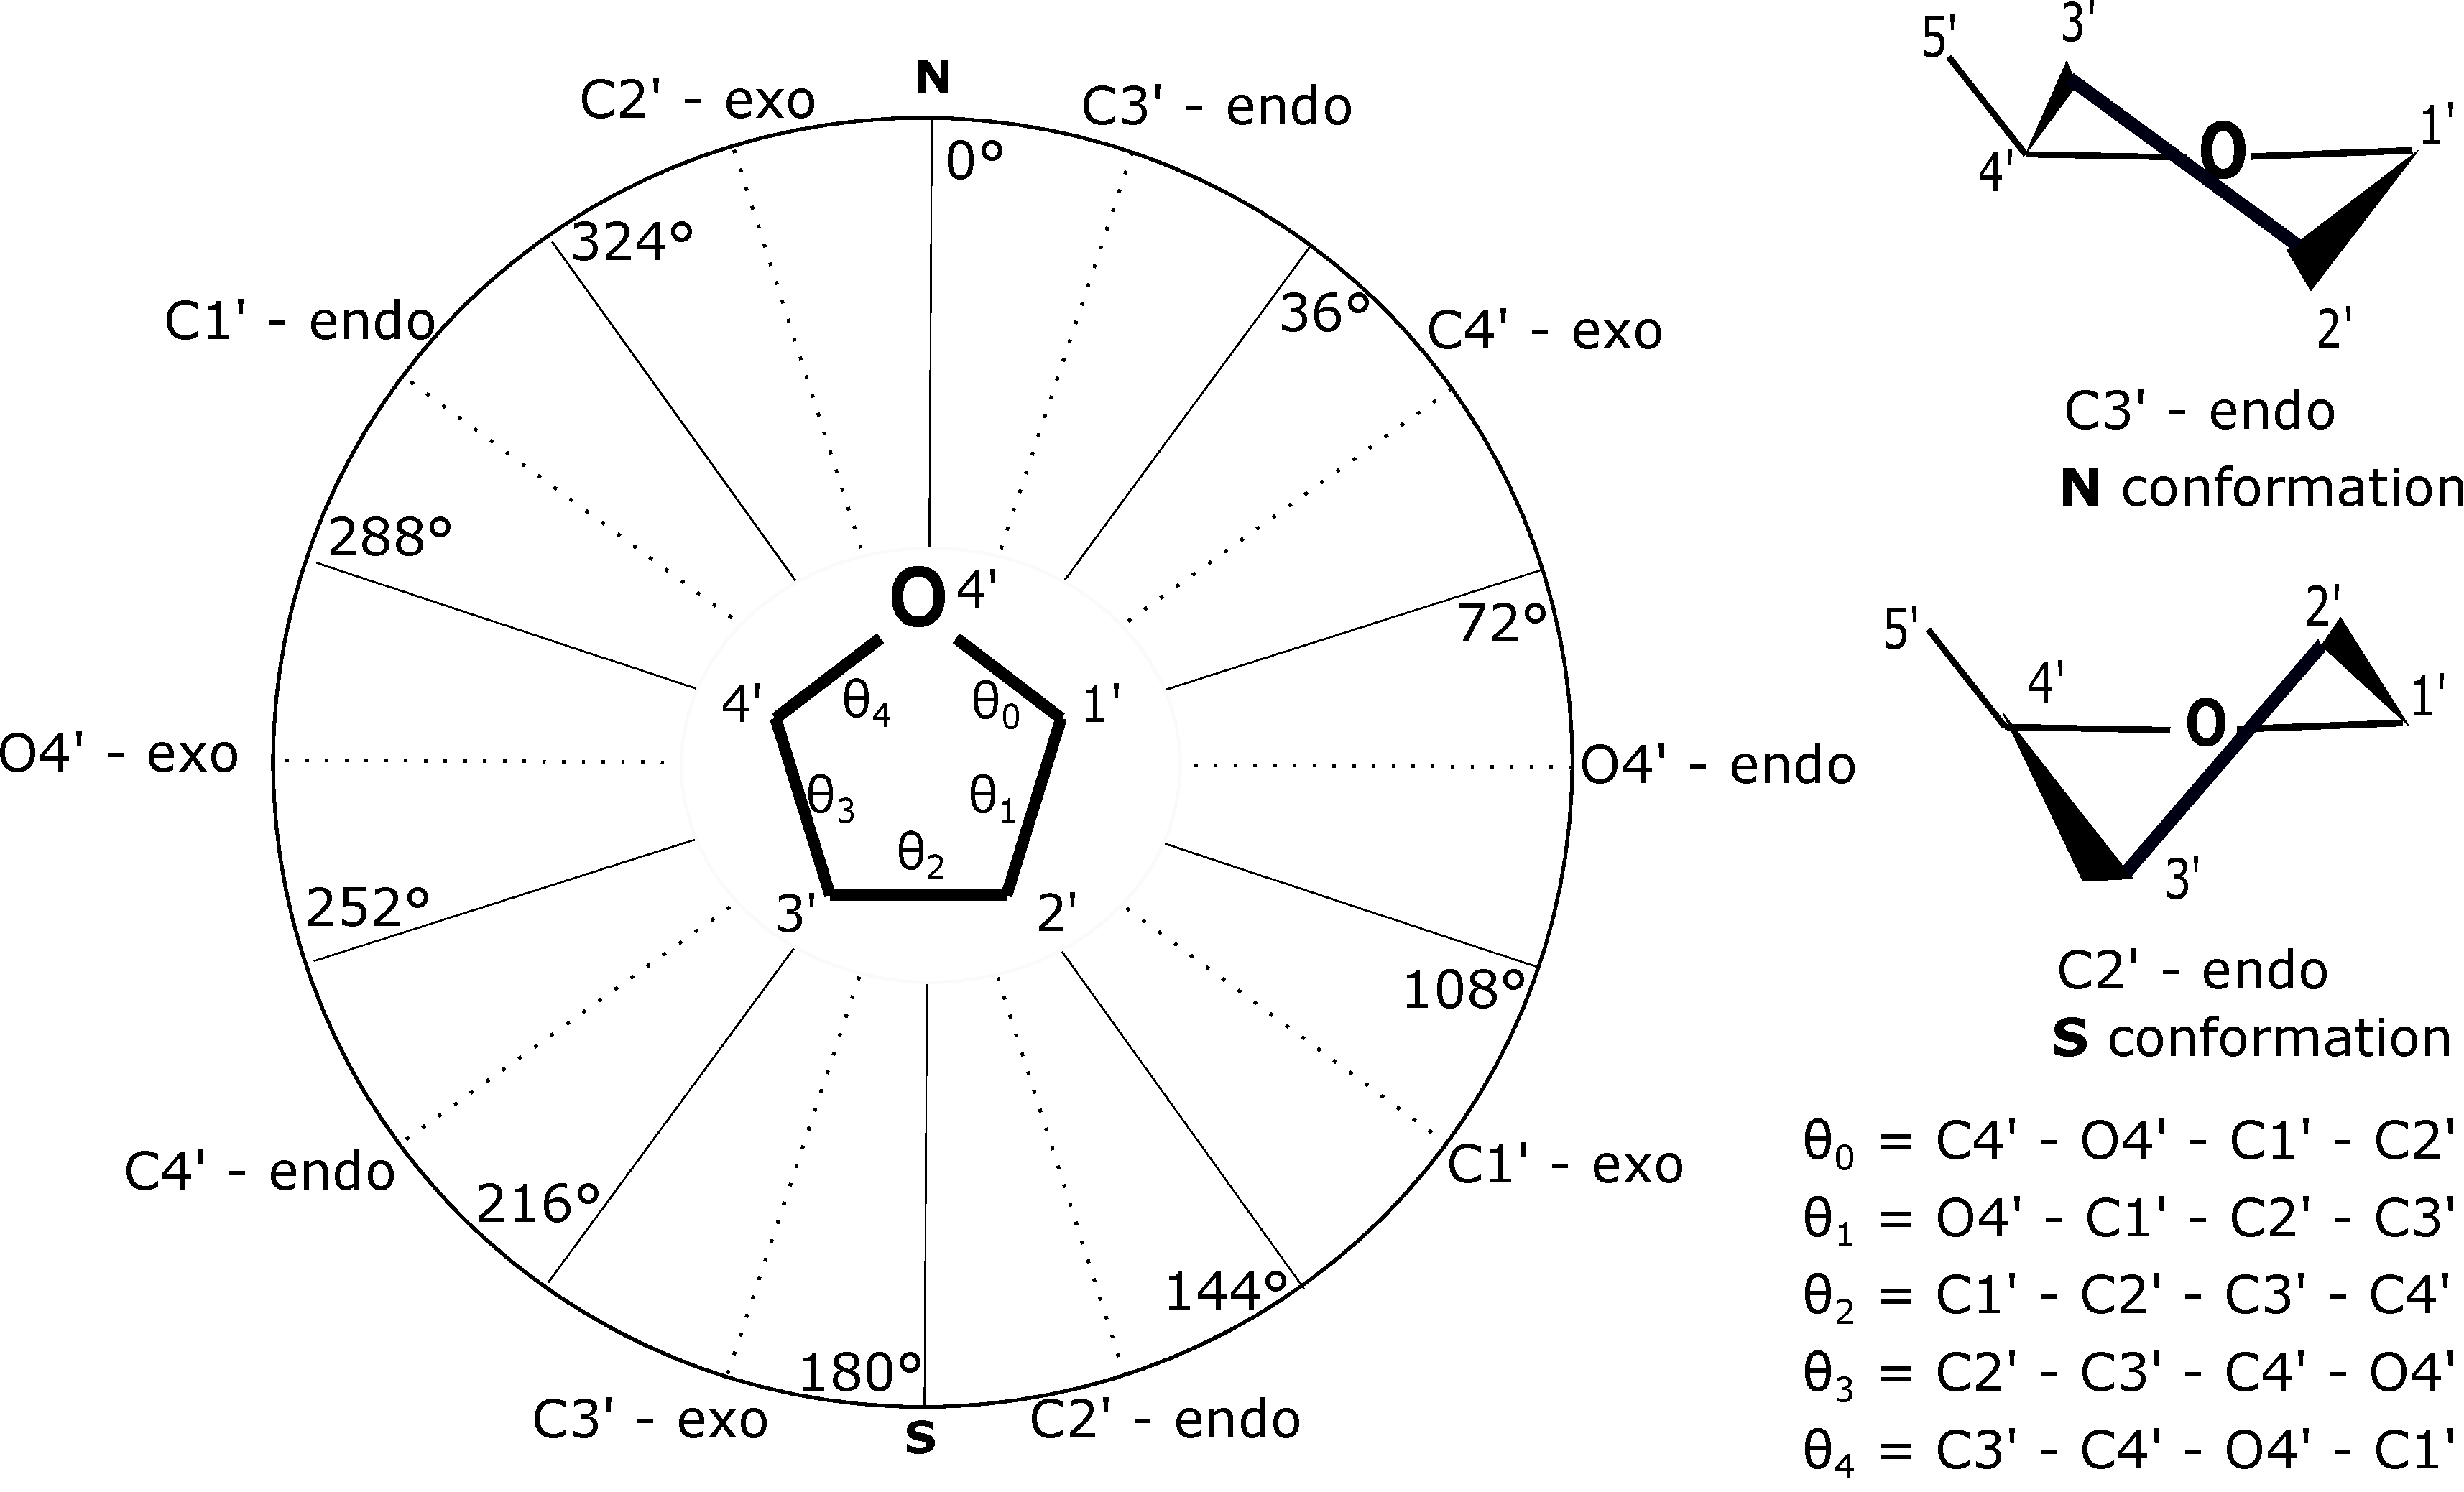
\includegraphics[scale=0.2]{images/pucker_mode.pdf}
	\centering\caption{
Pseudorotation wheel (on the left) adopted from ref.~\cite{altona1972conformational} with sugar pucker notations defined based on the pseudorotation phase angle (\textbf{\textsc{P}}). 
\textbf{\textsc{P}} is computed using various dihedral angles $\theta_i \; \forall \; i \in [0,1,2,3,4]$ as given in \cref{c1:eq1} and the label of atoms from which dihedral angles are computed is shown in the figure. 
The two most common conformations adopted by the sugar in DNA are shown on the left.
	}
\label{c1:fig4}
\end{center}
\end{figure}

%http://www.cactus.nci.nih.gov/prosit/
The deoxyribose sugar ring in DNA is inherently non-planar (due to ring strains) and adopts puckered conformations as shown in \cref{c1:fig4}. 
To fully describe the conformations of the sugar ring, five torsional angles are required.
The different ring torsional angles give rise to different puckered conformations, and the thermodynamic stability of these conformations is governed  
by the substituents on the ring carbon atoms and how far those substituents are from each other in a given puckered conformation. 
These puckered conformations can inter-convert into each other and can be concisely 
explained using two parameters~\cite{altona1972conformational}, namely, pseudorotation phase angle (\textbf{\textsc{P}}) and maximum degree of pucker, $\theta_{max}$
\begin{equation}
tan(\textbf{\textsc{P}}) = \frac{(\theta_4 + \theta_1) - (\theta_3 + \theta_0)}{2\theta_2\left(sin(36^\circ) + sin(72^\circ)\right)} \text{ and } \theta_{max} = \frac{\theta_{2}}{cos(\textbf{\textsc{P}})}
\label{c1:eq1}
\end{equation}
where \textbf{\textsc{P}} can be anything between $0-360^\circ$ and if $\theta_2 < 0$ then $\textbf{\textsc{P}} = \textbf{\textsc{P}} + 180^\circ$.
Now, puckered conformations corresponding to \textbf{\textsc{P}} can be best represented on a pseudo-rotation wheel, as shown in \cref{c1:fig4} with the description of $\theta_i \; \forall \; i \in [0,1,2,3,4]$. 

One of the most common pucker types is a conformation in which two of the ring atoms are out of the plane (on either side) formed by the other three atoms.
The name of such a conformation is based on the direction of major deviation of a non-planar atom, which is if on the opposite side as
C$4^\prime-$C$5^\prime$ bond and base, then the atom is called exo; otherwise, if it occurs in the same direction, then endo. 
The most frequently observed conformations are 
C$2^\prime-$endo (with \textbf{\textsc{P}} values $\in 140 \text{ to } 185^\circ$) or C$3^\prime-$endo (with \textbf{\textsc{P}} 
values $\in -10 \text{ to } +40^\circ$)~\cite{neidle2018principles} and are shown in \cref{c1:fig1}.
Even though various pucker modes of deoxyribose  are inter-convertible,
C$3^\prime-$endo pucker conformation is primarily dominated in the case of A-form DNA while
C$2^\prime-$endo in case of B-form DNA.
In these two conformations, C$2^\prime-$endo and C$3^\prime-$endo, the relative distance between the $3^\prime$ and $5^\prime$ phosphates as well as the orientation of the phosphate group with respect to base/sugar is significantly different, giving rise to very different A- and B-form of DNA. 

The DNA conformations are a function of the sequence, direction and amount of super-coiling, and the physical conditions of the solution. 
For example, the transition of B-DNA to A-DNA can be promoted under reduced humidity or by adding organic solvents.
DNA also exists in a few other forms, such as Z-DNA, which is a left-handed helical structure form in alternating RY tracts under high salt, the presence of certain divalent cations, or DNA super-coiling. 
Z-DNA is structurally quite different from B-DNA in terms of sugar puckering, glycosidic bond configuration, and relative bp orientation.
A concise summary of various DNA helical structures can be found in~\cite{ussery2002dna}. 

Compared to the DNA backbone, the bases are quite rigid and planar because of conjugation in the rings. 
We have heavily exploited this property of the bases by coarse-graining them. More details on this are discussed later in this thesis. 


\subsection{Ribonucleic Acid}\label{c1:s2:sb2}
The key chemical differences in RNA from DNA are a) the sugar molecule is ribose instead of deoxyribose and b) 
the pyrimidine base is U instead of T, as shown in \cref{c1:fig1}.
The ribose sugar preferably adopts C$3^\prime-$endo conformations, and the preferred geometry of the RNA is the A-form.
Discussion concerning the presence of two grooves, backbone, and sugar pucker modes analysis is analogous to DNA. 

\subsection{Epigenetic modifications in DNA}\label{c1:s2:sb3}
Most common epigenetic modifications in DNA are methylation or hydroxymethylation of Cytosine at the $5-$ position, as shown schematically in \cref{c1:fig1}.
Other base modifications, such as 5-formyl-C, 5-carboxyl-C, and N6-methyl-A, are comparatively rare in biology and are not studied in this work.
Most often, Cytosine substitution occurs at \cpg dinucleotide steps\cite{jabbari2004cytosine}, which can be di-substituted if both strands are symmetrically modified or hemi-substituted if only one of the strands is asymmetrically modified.
In this thesis, we have used the letter M for 5-methylated-Cytosine, and N for Guanine when the complementary Cytosine is methylated. 
Similarly, the letters H and K are used for 5- hydroxymethylated-Cytosine and Guanine complementary to 5-hydroxymethylated-Cytosine, respectively.

\subsection{DNA-RNA hybrid}\label{c1:s2:sb4}
A double-stranded DNA-RNA hybrid (abbreviated as DRH in this thesis) has one DNA strand and another RNA strand.
We always take the DNA strand as the Watson or reading strand for simplicity in writing and coding.
DRHs are important intermediates in many biological processes~\cite{adams2012biochemistry,vella1994molecular,rich1960hybrid,brambati2020dark,meselson1958replication,shaw2008recognition}. 
%For example, during reverse transcription, RNA viruses create transient DRH whose stability is consequential in their replication cycle~\cite{vella1994molecular}. 
%A detailed discussion on DRH formation and the influence on genome instability because it interferes with DNA replication and double-stranded DNA breaks repair can be found in this review~\cite{brambati2020dark}.
%Furthermore, DRHs are considered as potential medicinal agents for HIV and other retroviruses diseases~\cite{tisdale1991mutations,shaw2008recognition}. 
Compared to DNA and RNA, the structure and mechanics of DRH are much less explored.
Initial crystallographic studies indicated that DRH adopts a A-form geometry~\cite{wang1982molecular} but soon challenged by several other experimental techniques such as fiber diffraction~\cite{zimmerman1981rna}, circular dichroism~\cite{roberts1992stability},  NMR~\cite{gao1994sequence,lane1993nmr,fedoroff1997solution,szyperski1999nmr} finding a mix A- and B-form geometries in DRH. 
Moreover, NMR results suggested that the DNA strand adopts a geometry closer to the B-form while the RNA strand is close to the A-form geometry.
%One can also find a detailed account of DRH's structure and its role in biology in this review~\cite{shaw2008recognition}.
%Several MD simulations~\cite{cheatham1997molecular,noy2005structure,suresh2014dna,priyakumar2008atomic,liu2019structural} and theoretical studies~\cite{sanghani1994theoretical} supported the experimental findings of mix A- and B-form geometry in DRH with the DNA strand in B-like geometry with C2$^\prime-$endo sugar puckers while the RNA strand in A-like geometry with C3$^\prime-$endo sugar puckers.
Discussion concerning the presence of two grooves, backbone, and sugar pucker modes analysis is analogous to DNA. 

% RNAase H enzyme (crucial for genome stability and DNA replication of the mitochondrial genome~\cite{shaw2008recognition,brambati2020dark}) can selectively recognize DRH (among other double-stranded NAs) and degrade the RNA strand without affecting the complementary DNA strand~\cite{stein1969enzyme}.
% Experimental findings~\cite{fedoroff1997solution,szyperski1999nmr} attribute this selectivity of RNAase H enzyme to this intermediate minor groove width size as the key structural feature. Initially, the activity of this enzyme was considered to be sequence-independent while some recent experimental evidence suggested~\cite{huang1998structure,sarafianos2001crystal} otherwise with higher pu content in RNA strand leads to resistance in RNAase H enzyme activity.
% Moreover, in extensive studies by Modesto group~\cite{noy2005structure,noy2008theoretical} and Gorle et al.~\cite{suresh2014dna}, various sequence-dependent structural and mechanical factors such as helical coordinates, unique desolvation pattern, stability, and geometry of duplex, and enhanced conformational flexibility of DRH (from RNA) along with minor groove width has been proposed as the potential factors that affect the 
% activity of RNAase H enzyme.
% It highlights the importance of underlying sequence in the biological processes of DRH, unlike previously believed~\cite{fedoroff1997solution,szyperski1999nmr}.
% Elena et al.~\cite{lesnik1995relative} further demonstrated the sequence dependence in the thermodynamic stability HDR.%

\section{Methods}
\subsection{Sequence logos}\label{c1:sec_seq_logo}
Sequence logos~\cite{schneider1990sequence} are a popular graphical representation to plot sequence characteristics in DNA, RNA, or protein sequences. 
It is widely used to visualize sequence motifs in multiple sequence alignments. 
In sequence logos, each position has a stack of characters (A/T/C/G) on top of each other, with the character height proportional to the relative frequency of the nucleic base at that position, and the total height of the stacks tells the information content at that position. 
In this work, we have exploited this visualization technique to understand the role of sequence in dsNA mechanics.

In standard sequence logos, the height of the stack is the information content (in bits), which for nucleic acids (say DNA) is given as 
\begin{equation}
    \begin{split}
    H_i     &= \sum_{b}f_{b,i} \times log_2(f_{b,i}) \\
    R_i     &= 2 - H_i - e \\
    h_{b,i} &= f_{b,i} \times R_i
    \end{split}
\end{equation}
where $b \in$ \{A, T, C, G\}, $i$ is the $i^{\text{th}}$ position in the sequence, $H_i$ is the uncertainty or Shannon entropy at position $i$, $f_{b,i}$ is the frequency of $b^{\text{th}}$ base at position $i$, $R_i$ is the total information at position $i$ defined as the loss in uncertainty, and lastly, $h_{b,i}$ tells the height of base $b$ at position $i$. 
$e$ is a small sample correction taken as zero in this work. Note that the maximum value of $R_i$ can be 2, which implies no uncertainty at that position, and the minimum value is 0, which implies the highest uncertainty at that position, i.e., all possible b are equally probable. 


To better explain sequence logos, we have generated a set of sequences of length five bps.
In \cref{c1:seq_logo_demo}(top), we have plotted a variant of sequence logos with the y-axis as the probability of alphabet b at $i^{\text{th}}$ position.
In the bottom plot, we have plotted the corresponding standard sequence logos with information content (in bits) on the y-axis. 
From the probability plot, it can be observed that the uncertainty in base type increases from left to right. 
At position-1: all sequences have A, at position-2: 75\% G and 25\% C, and at position-5: all alphabets are equally probable. 
In the corresponding information content plot, left to right, the information decreases with position-1 containing the maximum and position-5 containing zero information. 
\begin{figure}[htb]
	\begin{center}
	\centering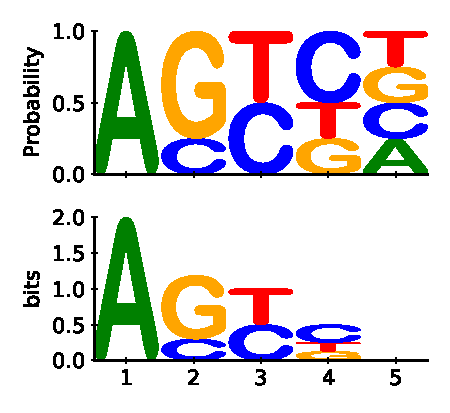
\includegraphics[scale=0.8]{images/demo_seq_logo.pdf}
	\centering\caption{Sequence logos plot for an artificial dataset with probability (top) and the information content (bottom) on the y-axis and base position in the sequence on the x-axis.}
\label{c1:seq_logo_demo}
\end{center}
\end{figure}

%In the minor groove, N3 of A or G and O2 of T or C can serve as hydrogen acceptors, and the amino group attached to C2 of G can be a hydrogen donor. 
%In the major groove, N7 of G or A is a potential acceptor, as are O4 of T and O6 of G. 
%The amino groups attached to C6 of A and C4 of C can serve as H-donors. 
%Note that the major groove displays more features that distinguish one base-pair from another than the minor groove. 
%The larger size of the major groove in B-DNA makes it more accessible for interactions with proteins that recognize specific DNA sequences.

\section{Codes and data availability}
Details of all the codes and data used in this thesis are provided \cref{app6}. 

